\documentclass[11pt,letterpaper]{article}
\pdfinfoomitdate=1
\pdftrailerid{}
\pdfsuppressptexinfo=15
\usepackage[margin=0.93in]{geometry}
\usepackage{graphicx}
\setlength{\textfloatsep}{10pt plus 2pt minus 2pt}
% Decimal display values for the journal draft.
% The upper macro may be replaced by a certified decimal after independent review.
\newcommand{\CstarLower}{0.1405694688}
\newcommand{\CstarUpper}{\textbf{[certified upper bound pending]}}
\newcommand{\QuadraticExponent}{2}

\usepackage{amsmath,amssymb,amsthm,booktabs,longtable}
\usepackage[hidelinks]{hyperref}
\usepackage[T1]{fontenc}
\usepackage{lmodern}
\usepackage[mathlines]{lineno}
\emergencystretch=1em
\hypersetup{pdftitle={The quadratic growth of the minimum central circle},
 pdfauthor={Maurizio Falconi}}
\newtheorem{theorem}{Theorem}
\newtheorem{lemma}[theorem]{Lemma}
\newtheorem{proposition}[theorem]{Proposition}
\newtheorem{corollary}[theorem]{Corollary}
\theoremstyle{definition}\newtheorem{definition}[theorem]{Definition}
\theoremstyle{remark}\newtheorem{remark}[theorem]{Remark}
\newcommand{\Rstar}{R^\ast}
\newcommand{\ch}{R_{\mathrm{chain}}}
\newcommand{\full}{R_{\mathrm{full}}}
\newcommand{\CC}{C_\ast}
\DeclareMathOperator{\atan}{arctan}
\DeclareMathOperator{\asin}{arcsin}
\title{The quadratic growth of the minimum central circle}
\author{Maurizio Falconi}
\date{3 November 2026}
\begin{document}
\maketitle
\nolinenumbers
\begin{abstract}
For outer circles of consecutive positive integer radii up to $n$, the
minimum radius of a central circle tangent to them all satisfies
$\Rstar(n)=\CC n^{\QuadraticExponent}+o(n^{\QuadraticExponent})$ as $n\to\infty$.
The bracket for the limiting coefficient is
$\CstarLower<\CC<\CstarUpper$.
An exact angular comparison reduces the problem to marked points on a line
whose pairwise separations are bounded below by the geometric mean of
their marks. Finite placements can be joined and their marks reassigned
to the prescribed radii, giving a limit over all sizes and cyclic orders.
A linear program on words of fixed length characterizes this limit with
an explicit error for both mark discretization and word boundaries.
A coupled estimate on terminal subsets supplies the lower endpoint.
Reflected blocks yield upper constructions realized by actual
circle placements satisfying every pair constraint.
\end{abstract}
\noindent\textbf{Keywords:} circle packing; geometric optimization; asymptotic
limits; linear programming; rigorous computation.
\par\noindent\textbf{MSC 2020:} 52C15, 52C26, 90C05.


\section{The minimum central circle}

Place circles of radii $1,\ldots,n$ around a central circle, all externally
tangent to it and with pairwise disjoint interiors. For an outer cyclic
order $\sigma$, let $\full(\sigma)$ be the least feasible central radius.
We seek the growth of $\Rstar(n)=\min_\sigma\full(\sigma)$. The adjacent
chain closure $\ch(\sigma)$ gives a lower bound on $\full(\sigma)$.
Paper~I~\cite{paperI} treats the ordering of these chains and certifies
the global finite optima for $3\le n\le14$ by tight brackets.

\paragraph{Main results.}
Theorem~\ref{thm:existence} identifies $\pi\CC$ with the limiting mean
span of a line placement and with an infimum over finite templates.
Theorem~\ref{thm:lp} encloses $\CC$ by a finite linear program with
error width $(1/k+1/r)/\pi$ for $k$ types and words of length $r$.
The explicit lower bound in Proposition~\ref{prop:lower} exceeds $1/8$
and disproves the coefficient conjectured in Paper~I~\cite{paperI}.
For the upper endpoint, Theorem~\ref{thm:blocks} recovers feasible
finite permutations from reflected-block measures with a quantitative
error. Together the endpoint arguments give
$C_{\rm term}+\eta_{\rm width}\le\CC\le U_4$ (Proposition~\ref{prop:lower}
and~\eqref{eq:U4}).

\paragraph{Related work.}
Alt et al.~\cite{shelf} study disks resting on a shelf and minimizing
the width of their horizontal envelope. Their geometric-mean separation
rule gives the line problem in Definition~\ref{def:line} (Figure~\ref{fig:line}).
For marks at most one, that envelope differs from
$2(\max_i x_i-\min_i x_i)$ by at most two.
Klemz, N\"ollenburg and Prutkin~\cite{contact} study weighted disk
contact graphs, where a prescribed graph specifies the tangencies. In
the central-circle problem all spokes are required and the outer
contacts are free. For a fixed order, angular feasibility has a
difference-constraint formulation in Paper~I, in the framework of
temporal constraint networks~\cite{temporal}. The chain-order result
of Paper~I uses Supnick's structured traveling-salesman
problem~\cite{supnick}, part of the class of tractable cases surveyed
by Burkard et al.~\cite{burkard}.

The shortest-tour theorem of Beardwood, Halton and Hammersley~\cite{bhh}
also identifies a leading geometric optimization constant, for randomly
sampled points. Steele~\cite{steele} develops probabilistic approaches
to combinatorial optimization. Here every size has its own deterministic
set of labels. The finite-type argument uses the elementary subadditivity
lemma~\cite[Theorem~4.9]{walters}, while the passage between different
label sets requires reassignment in Theorem~\ref{thm:existence}.
The use of verified arithmetic for finite inequalities follows the
distinction between numerical approximation and certified bounds
developed by Rump~\cite{rump} and Tucker~\cite{tucker}.

\section{Exact Angular Comparison}\label{sec:line}

The cosine law gives the required pair angle
\begin{equation}\label{eq:theta}
 \theta_R(u,v)=2\asin\sqrt{\frac{uv}{(R+u)(R+v)}}
 =2\atan\sqrt{\frac{uv}{R(R+u+v)}}.
\end{equation}
Both directed cyclic arcs between a pair must be at least this angle.
This is equivalent to non-overlap, since their smaller separation belongs
to $[0,\pi]$. The angle is positive, symmetric, increasing in either
outer radius and strictly decreasing in $R>0$.
For a cyclic order $\sigma=(u_1,\ldots,u_n)$, $n\ge3$, with $u_{n+1}=u_1$,
$\ch(\sigma)$ is the unique positive root of
$\sum_{i=1}^n\theta_R(u_i,u_{i+1})=2\pi$.
Indeed, the sum decreases continuously from $n\pi$ to zero. Summing the
adjacent constraints in any full placement proves $\ch(\sigma)\le\full(\sigma)$.

We next introduce an auxiliary problem on a line. Its comparison with the
circle problem will follow after a bound on the cost of closing a line
placement.

\begin{definition}\label{def:line}
For a finite multiset $a=(a_1,\ldots,a_N)$ of marks in $[0,1]$, let $b(a)$
be the least span of a line placement satisfying
\begin{equation}\label{eq:line}
 |x_i-x_j|\ge\sqrt{a_i a_j}\quad(i\ne j).
\end{equation}
Distinct zero-mark points may coincide. Write $b_n=b(1/n,2/n,\ldots,1)$.
\end{definition}

\begin{figure}[tb]
\centering
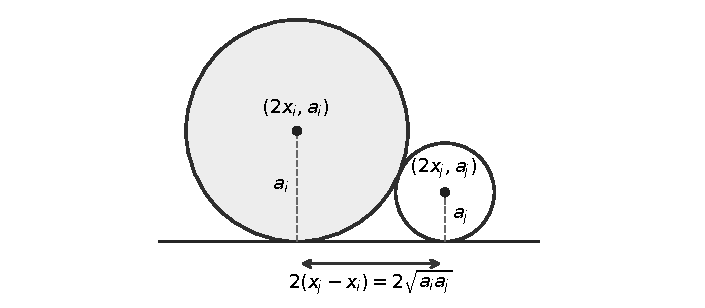
\includegraphics[width=.65\linewidth]{figures/line_geometry.pdf}
\caption{Two disks tangent to the same line. Their center separation
squared is $4(x_j-x_i)^2+(a_j-a_i)^2$. At contact this equals
$(a_i+a_j)^2$, giving equality in~\eqref{eq:line}.}
\label{fig:line}
\end{figure}

For a fixed word $w=(w_1,\ldots,w_N)$ in left-to-right order, its minimum
span $\ell(w)$ is attained by
\begin{equation}\label{eq:recurrence}
 x_1=0,\qquad x_i=\max_{j<i}\{x_j+\sqrt{w_iw_j}\},\qquad \ell(w)=x_N.
\end{equation}
Induction proves that these coordinates are componentwise no larger than
any feasible ordered coordinates with $x_1=0$; they also satisfy every
constraint. Nonnegative weights ensure ordered coordinates. Equivalently,
$\ell(w)$ is the longest increasing-index path from $1$ to $N$, with
edge weight $\sqrt{w_iw_j}$. Thus $b(a)$ is an attained minimum over a
finite set of orders. Deleting or decreasing marks cannot increase it;
scaling all marks by $h$ scales the minimum span by $h$.

\begin{lemma}[Bounded closing cost]\label{lem:closing}
Let $B(a)$ be the infimum circumference with both pair arcs at least
$\sqrt{a_i a_j}$. Then $b(a)\le B(a)\le b(a)+1$.
\end{lemma}
\begin{proof}
Cut a feasible circle to obtain a feasible line placement. Conversely,
close a feasible line placement by an additional gap of length one. One
arc for every pair is its line separation; the other contains the added
gap and is at least $1\ge\sqrt{a_i a_j}$. Both arcs are controlled.
\end{proof}

\begin{lemma}[Exact geometric squeeze]\label{lem:squeeze}
For every $n\ge3$,
\begin{equation}\label{eq:squeeze}
 \frac{b_n}{\pi n}-\frac1n
 \le\frac{\Rstar(n)}{n^2}\le\frac{b_n+1}{\pi n}.
\end{equation}
\end{lemma}
\begin{proof}
For $1\le u,v\le n$, the two expressions in \eqref{eq:theta} give
\[
 \frac{2\sqrt{uv}}{R+n}\le\theta_R(u,v)\le\frac{2\sqrt{uv}}R.
\]
The first uses $\asin z\ge z$ and
$\sqrt{(R+u)(R+v)}\le R+n$; the second uses $\atan z\le z$.
Scaling a feasible ring's angles by $(R+n)/(2n)$ gives a feasible linear
circle of circumference $\pi(R+n)/n$, proving the lower inequality.
Conversely, the circumference $b_n+1$ from Lemma~\ref{lem:closing},
scaled to $2\pi$, satisfies every original pair angle at
$R=n(b_n+1)/\pi$. This proves the upper inequality. No Taylor expansion,
adjacency reduction or assumption on the optimal order was used.
\end{proof}

\section{Existence by Genuine-Label Concatenation}

The closing estimate makes concatenation useful: copies of a finite line
placement can be joined at bounded cost. The next theorem combines this
construction with reassignment to the prescribed normalized radii.

\begin{theorem}[The leading limit exists]\label{thm:existence}
There is a constant $\CC$ such that
\begin{equation}\label{eq:limit}
 \Rstar(n)=\CC n^2+o(n^2),\qquad
 \pi\CC=E:=\lim_{n\to\infty}\frac{b_n}{n}
 =\inf_{n\ge2}\frac{b_n+1}{n}.
\end{equation}
\end{theorem}
\begin{proof}
Copies of a feasible line template, separated by unit gaps, satisfy all
cross-copy constraints as well as the internal ones. Fix $n\ge2$. Given
$N\ge n$, let $q=\lceil N/n\rceil$ and concatenate $q$ copies of an
optimal $b_n$ template. Its span is $q(b_n+1)-1$.
Retain the $N$ smallest marks. The $i$th sorted retained mark is
$\lceil i/q\rceil/n$. Scale all marks and coordinates by $h=nq/N$.
The resulting $i$th mark is at least $i/N$, so decreasing it to $i/N$
preserves every constraint. Each target label is assigned exactly once
to an actual retained point, with ties broken arbitrarily. Hence
\begin{equation}\label{eq:copies}
 b_N\le\frac{nq}{N}\bigl[q(b_n+1)-1\bigr].
\end{equation}
Intermediate marks exceeding one cause no problem: the line inequalities
are homogeneous, and final marks are exactly $1/N,\ldots,1$.

As $N\to\infty$, $q/N\to1/n$, giving
$\limsup_N b_N/N\le(b_n+1)/n$ for every fixed $n$.
The sequence is bounded between zero and one by equally spaced placements.
Taking $n$ along a subsequence attaining its liminf gives equality of
limsup and liminf. Taking the infimum and then $n\to\infty$ proves
the last equality in \eqref{eq:limit}. Lemma~\ref{lem:squeeze} transfers
the limit to the original ring problem for all sizes and both parities.
Finally, at least $n/2$ marks are at least $1/2$. Their successive line
separations are at least $1/2$, so $E\ge1/4$ and $\CC>0$.
\end{proof}

\section{A finite linear-programming characterization}\label{sec:lp}

We now turn from existence of the limit to approximation with a prescribed
error. There are two steps: replace the radii by finitely many types, then
replace long orderings by distributions of finite words. Each step contributes
one term to the bracket width.

\subsection{Finite Types and a Uniform Quantization Error}
For $k\ge1$, let $A_{k,q}$ contain $q$ copies of each mark
$1/k,\ldots,1$, and let $A^-_{k,q}$ instead contain $q$ copies of
$0,1/k,\ldots,(k-1)/k$. Define
$e_k=\lim_{q\to\infty}b(A_{k,q})/(kq)$ and
$e^-_k=\lim_{q\to\infty}b(A^-_{k,q})/(kq)$; these limits exist.
Indeed $a_q=b(A_{k,q})+1$ is subadditive by unit-gap concatenation.
Writing $q=hp+s$ at fixed $p$ proves
$\limsup a_q/q\le a_p/p$; then taking $p$ along a liminf subsequence
proves the limit. The same argument applies to the lower types.

The two multisets share every nonzero type except the top type. Zero marks
cost nothing. Adding the $q$ unit marks as a separate equally spaced
block costs at most $q$, including the join. Thus, also for $k=1$,
\[
 e^-_k\le e_k\le e^-_k+\frac1k.
\]
For $n=kq$, the sorted uniform marks $i/n$ lie between the two sorted
type multisets. Theorem~\ref{thm:existence} and monotonicity imply
\begin{equation}\label{eq:types}
 e_k-\frac1k\le E\le e_k.
\end{equation}

\subsection{Balanced Words and the Quantified Boundary Relaxation}
A word records a short consecutive piece of an ordering. The linear program
balances type counts across a distribution of words; the proof below controls
the cost of joining them.

Fix $k\ge1$ and $r\ge2$, and use all $k^r$ words
$w\in\{1/k,\ldots,1\}^r$, including repetitions. Let $c_j(w)$ count
occurrences of $j/k$. Compute $\ell(w)$ by \eqref{eq:recurrence}, and define
\begin{equation}\label{eq:lp}
\begin{split}
 \lambda_{k,r}=\min_p\ &\frac1r\sum_w p_w\ell(w),\\
 p_w\ge0,\quad &\sum_w p_w=1,\quad
 \sum_w p_wc_j(w)=\frac rk\quad(1\le j\le k).
\end{split}
\end{equation}
The polytope is nonempty: equally mix the $k$ constant words.

\begin{theorem}[Finite linear-programming bounds]\label{thm:lp}
For every $k\ge1,r\ge2$,
\begin{equation}\label{eq:effective}
 \boxed{\quad\frac{\lambda_{k,r}-1/k}{\pi}\le\CC
 \le\frac{\lambda_{k,r}+1/r}{\pi}\quad}.
\end{equation}
Consequently $\CC=\pi^{-1}\lim_{k,r\to\infty}\lambda_{k,r}$, jointly,
with certified bracket width $(1/k+1/r)/\pi$.
\end{theorem}
\begin{proof}
Partition an optimal ordering of $A_{k,q}$ into consecutive blocks of
$r$ vertices, discarding fewer than $r$ leftover vertices. Their spans
sum to at most the full span and each is at least its word cost.
Empirical word distributions have convergent subsequences in the finite
simplex. Their limiting mean type counts are $r/k$, since the discarded
counts vanish after normalization. Hence $\lambda_{k,r}\le e_k$.

Conversely, the rational feasible polytope in \eqref{eq:lp} has a minimizing
rational vertex even though its cost entries are algebraic. Choose a
common denominator $D$. A batch with $Dp_w$ copies of each word has
exactly $Dr/k$ copies of each type, an integer by the count constraints.
Place every word at its minimum span and separate blocks by unit gaps.
All within-block and cross-block pairs are feasible. Repeating batches
gives asymptotic mean span
$\sum_w p_w(\ell(w)+1)/r=\lambda_{k,r}+1/r$.
The finite-type limit therefore satisfies
$e_k\le\lambda_{k,r}+1/r$. Combine with \eqref{eq:types}.
\end{proof}

\subsection{Exact Certificates and Computational Meaning}
Directed rational square-root enclosures of width $\epsilon$ give
word-span enclosures of width at most $(r-1)\epsilon$: every path in
\eqref{eq:recurrence} has at most $r-1$ edges. Rational endpoint LPs
then enclose $\lambda_{k,r}$ with additional width at most
$(r-1)\epsilon/r$. They can be solved by finite exact vertex enumeration.
Practical solvers may instead find solutions for subsequent exact verification.
For a rational lower cost $\ell^-(w)$, dual coefficients satisfying
\[
 y_0+\sum_j y_jc_j(w)\le\ell^-(w)/r\quad\hbox{for every word}
\]
certify the lower value $y_0+(r/k)\sum_jy_j$. Feasible rational $p$
certifies an upper value using upper costs. All such checks are finite
rational comparisons; equality is not decided by indefinite interval
refinement. Together with a rational enclosure of $\pi$, this proves
arbitrary-precision computability of $\CC$ in principle.

For example, $k=r=64$ gives width $1/(32\pi)<0.01$ before directed
arithmetic error, with $64^{64}$ words in the displayed formulation.
The endpoint constructions below provide bounds directly.

\section{Explicit Geometric Upper Constructions}\label{sec:upper}

The finite-word characterization gives a convergent scheme for the constant.
For explicit upper bounds, we use reflected-block constructions
(Figure~\ref{fig:cells}). The key step
is to recover actual permutations satisfying every pair constraint from the
continuous description.

\begin{figure}[tb]
\centering
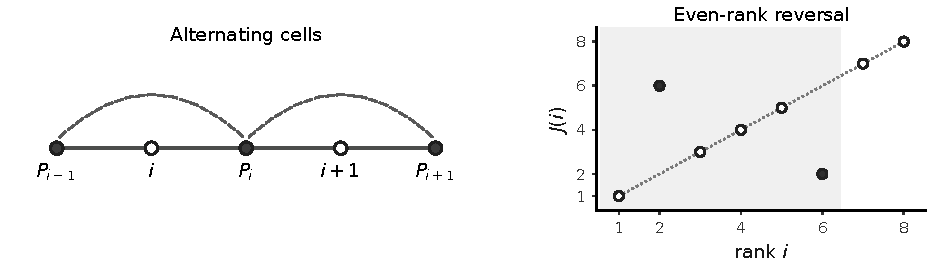
\includegraphics[width=.84\linewidth]{figures/reflected_cells.pdf}
\caption{Left, filled vertices denote high labels and open vertices low labels.
Each cell must accommodate the solid high--low--high path and the dashed
direct high-pair constraint. Right, one six-rank slab reverses its even
ranks before the cyclic high-label shift. Ranks outside the slab stay fixed.}
\label{fig:cells}
\end{figure}

Fix $0\le\alpha<1$ and nonnegative adjacent slab lengths
$\ell_1,\ldots,\ell_k$ of total $T<1-\alpha$. Put $A=1+\alpha$,
$t_0=0$, $t_j=\sum_{h\le j}\ell_h$. On each slab
$[t_{j-1},t_j]$, use equal masses at
\[
 (t,A+t,A+t_{j-1}+t_j-t),\qquad
 (t,A+t_{j-1}+t_j-t,A+t).
\]
After $T$, use the diagonal $(t,1+\{t+\alpha\},1+\{t+\alpha\})$.
This defines a measure $\mu$ on $[0,1]\times[1,2]^2$ with uniform low
and separate high marginals. Its complete cell cost is
\begin{equation}\label{eq:blockcost}
 C(\mu)=\frac1{4\pi}\int
 \max\{\sqrt t(\sqrt X+\sqrt Y),\sqrt{XY}\}\,d\mu.
\end{equation}
Correct marginals alone do not establish finite recovery.

\begin{theorem}[General block transfer]\label{thm:blocks}
Every such finite partition has genuine alternating-half permutations with
all-pairs-feasible radii $\rho_m=\full(\sigma_m)$ and
\[
 \left|\frac{\rho_m}{(2m)^2}-C(\mu)\right|
 \le\frac{(6k^2+28k+1060)/m+16384/(3m^2)}{4\pi}
\]
for $m\ge\max\{2048,\lceil2/(1-\alpha-T)\rceil\}$.
It follows that $\CC\le C(\mu)$. Countably many slabs also transfer
if their total length is strictly below $1-\alpha$.
\end{theorem}
\begin{proof}[Proof with explicit construction]
Let $s=\lfloor\alpha m\rfloor$, $l_j=2\lfloor\ell_jm/2\rfloor$,
$a_0=0$ and $a_j=\sum_{h\le j}l_h$. Reverse only the even ranks within
each $(a_{j-1},a_j]$ to obtain a permutation $J$ of $\{1,\ldots,m\}$.
Set $J(i)=i$ on odd ranks and on every index outside these blocks.
Set $P_i=m+1+((J(i)+s-1)\bmod m)$ and
$\sigma_m=(1,P_1,\ldots,m,P_m)$, with $P_0=P_m$.
Disjoint involutions and the cyclic shift prove bijectivity, including
zero blocks and length-two identities. The lower bound on $m$ keeps the final
block endpoint at least two ranks before the high wrap, and its exit
strictly before that wrap.

Double panels of width $2/m$, allocated half to each parity, recover
the two reflected orientations. Interior coordinate error is at most
$4/m$. There are at most $k+3$ exceptional actual cells: shared exits,
the cyclic predecessor, and the two wrap cells. Rounded slab boundaries
and wrap differ on a set of length at most $[k(k+1)+1]/m$, with remaining
coordinate error at most $(4k-1)/m$. Write
$g(t,X,Y)=\max\{\sqrt t(\sqrt X+\sqrt Y),\sqrt{XY}\}$ for the integrand
in \eqref{eq:blockcost}. It is $4$-Lipschitz and lies in $[1,3)$.
The actual normalized full-cell moment is
\[
 G_m=\frac1m\sum_{i=1}^m g(i/m,P_{i-1}/m,P_i/m).
\]
It differs from
$\int g\,d\mu$ by at most $(6k^2+28k+36)/m$.

For arbitrary distinct highs in $[m+1,2m]$, the exact full-feasibility
criterion for this alternating order is
\[
 \sum_{i=1}^m\max\{\theta_R(P_{i-1},i)+\theta_R(i,P_i),
                         \theta_R(P_{i-1},P_i)\}\le2\pi.
\]
Its sufficiency follows from the high-shell triangle inequality
$2\theta_R(m+1,m+1)>\theta_R(2m,2m)$ and high/low separation:
each directed high path contracts through whole cells, and paths with
low endpoints either contain such a high path or an incident high gap
that already exceeds the endpoint requirement. Both directions are
treated separately. At its unique root, choose the first half of each
cell at its required low/high angle and put any excess in the other half.
This closes at $2\pi$ and satisfies all pairs.

At $R=4cm^2$, $c\ge1/32$, the full score differs from $G_m/(2c)$ by
at most $1024/m+16384/(3m^2)$. For $m\ge2048$ this first brackets
the actual normalized root in $(1/32,1/2)$, then yields the stated error.
Deleting label $2m$ gives the odd upper bound. For countably many slabs,
truncate and use that the omitted complete-cost integral is at most six
times the omitted length. A diagonal sequence with $m$ growing faster
than $k^3$ pays both finite and tail errors. Full cell/seam formulas and
the angle estimate are supplied in the upper supplement S2 of~\cite{supp}.
\end{proof}

For the explicit four-block construction, let $x_*$ be the unique minimizer
on $[0,1]$ of
\[
 E(x)=\int_0^x\!\left[
 \max\{\sqrt{(1+t)(1+x-t)},\sqrt t(\sqrt{1+t}+\sqrt{1+x-t})\}
 -\max\{1+t,2\sqrt{t(1+t)}\}\right]dt.
\]
Let $K(\alpha)=\int_0^1\max\{\sqrt{t h_\alpha(t)},h_\alpha(t)/2\}\,dt$,
where $h_\alpha(t)=1+\{t+\alpha\}$, and let $\widehat\alpha$ be the
unique zero of $K'(\alpha)+(1+\alpha)E(x_*)$ on $[0,1/2]$.
Set $A=1+\widehat\alpha$ and $\lambda=Ax_*$.
The second width $\epsilon_b$ is the unique mixed-branch stationary
minimum for a separate reflection starting at $\lambda$; the third width
$\Delta_*$ is the analogous unique minimum starting at
$v=\lambda+\epsilon_b$. Each width is minimized over
$[0,A/3-u]$ at its fixed start $u$, retaining the full max.
Supplement S2 of~\cite{supp} gives their exact defining integrals,
existence/uniqueness proofs and rational isolations:
\[
\begin{gathered}
 .1093<\widehat\alpha<.10931,\qquad .2876<x_*<.2877,\\
 .043<\epsilon_b<7/160,\qquad 29/5000<\Delta_*<27/4000.
\end{gathered}
\]
These terminating decimals are rational bracket endpoints, not definitions
or numerical replacements for the parameters.

Let $C_3(d)$ be \eqref{eq:blockcost} for the three lengths
$(\lambda,\epsilon_b,d)$, and $C_4(\eta)$ the same cost for the four
lengths $(\lambda,\epsilon_b,\Delta_*,\eta)$.
Use $\eta=1/20000$ and define $U_4=C_4(1/20000)$.
If $w=\lambda+\epsilon_b+\Delta_*$, $B=A+w$ and
$M=B+\eta/2$, the fourth increment at $0<\eta\le1/20000$ is exactly
\[
 C_4(\eta)-C_3(\Delta_*)=
 -\frac1{4\pi}\int_{-\eta/2}^{\eta/2}
       \frac{z^2}{M+\sqrt{M^2-z^2}}\,dz.
\]
Rational input margins keep both changed maxima strictly chord.
Since $2B\le M+\sqrt{M^2-z^2}\le2M$, $M<3/2$ and $\pi<4$,
\begin{equation}\label{eq:U4}
 \CC\le U_4<C_3(\Delta_*)-\frac1{4608000000000000}.
\end{equation}
The leading decrement is $-\eta^3/(96\pi B)$, with remainder between
zero and $\eta^4/(192\pi B^2)$. The theorem transfers this literal
continuous saving to genuine full geometry. It does not make four blocks
globally optimal or optimize an infinite partition.

\section{An Explicit Global Lower Endpoint}

Define $\tau$ as the unique root of $\cos\tau=\tau$ in $(0,1)$, set
$q=(1-\sin\tau)/(1+\sin\tau)$ and
$C_{\rm term}=\tau(1+q)/(2\pi)$.
For the fixed cutoffs
\[
 (\beta_1,\beta_2,\beta_3)=(2091/10000,10907/50000,23/100)
\]
put
\[
 D_i=\int_q^{\beta_i}[1+q-x-2\sqrt{x(1+q-x)}]\,dx,
 \quad F(h)=\sum_i h_iD_i-8\sum_i h_i^3.
\]
Let $a=113/12500$, $b=593/50000$. On
$h_i\ge0$, $h_1+h_2\le a$, $h_2+h_3\le b$, define
\[
 \eta_{\rm width}=\max_h
 \frac{\max\{F(h),0\}}{\pi(16+432\sum_i h_i)}.
\]
This maximum is uniquely attained at $(a-z_*,z_*,b-z_*)$, where $z_*$
is the unique zero on $[0,a]$ of $G=N'L+432N$,
$N(z)=F(a-z,z,b-z)$ and $L(z)=16+432(a+b-z)$.

\begin{proposition}[Explicit global lower bound]\label{prop:lower}
The global constant satisfies $\CC\ge C_{\rm term}+\eta_{\rm width}$,
with exact directed enclosure
\[
 .14056946887766098063257
 < C_{\rm term}+\eta_{\rm width}
 < .14056946887766098063392.
\]
In particular $\CC>1/8$, ruling out the proposed coefficient
and the stronger estimate $n^2/8-\Rstar(n)=O(\sqrt n)$.
\end{proposition}
\begin{proof}[Proof outline]
The complete proof L1--L8 and exact arithmetic certificates are in the
standalone lower supplement S1 of~\cite{supp}.
Its essential coupled information is one shared crossing energy for the
same order and all three nested terminal restrictions. An explicit assignment
dual bounds the reflected-grid energy by eight times the excess chain cost.
The absolute signed deletion discrepancy at cutoff $i$ is at most $54$
times this energy plus twice its crossing term. Separated strips charge
the common energy once, yielding
the scalar gain $\max\{F(h),0\}/(16+432\sum h_i)$.
The exact angular squeeze transfers each induced chain bound to any original
full feasible configuration. Uniform finite errors vanish at every fixed
strictly separated width vector.

For the width optimum, $G'<0$ and rational endpoint bounds isolate its zero.
Set $u=(a-z_*,z_*,b-z_*)$, $\mathcal L(h)=16+432\sum_i h_i$ and
$\rho=F(u)/\mathcal L(u)$. The gradient of $F-\rho\mathcal L$ at $u$ is a positive
combination of the two constraint normals. Its exact remainder is
$-8\sum_i(h_i-u_i)^2(h_i+2u_i)$, proving global uniqueness on the whole
closed region. To pass to the geometric limit, first use $tu$ at fixed
$0<t<1$, take $n\to\infty$, then $t\uparrow1$. The boundary
widths fail finite floor separation infinitely often; the proof never uses
them as an eventual finite separation condition. The uniform finite error bounds for this
limiting argument are supplied in S1 of~\cite{supp}. The result does not assert
that this particular lower mechanism reaches $\CC$.
\end{proof}

\section{Finite values and open questions}

Figure~\ref{fig:finite} compares the twelve finite brackets with the
lower bound for the limit. The proofs of existence and of the
linear-programming bracket use the angular model and genuine labels
directly. The values of $n$ in the figure illustrate how finite optima
compare with the limiting scale.

\begin{figure}[tb]
\centering
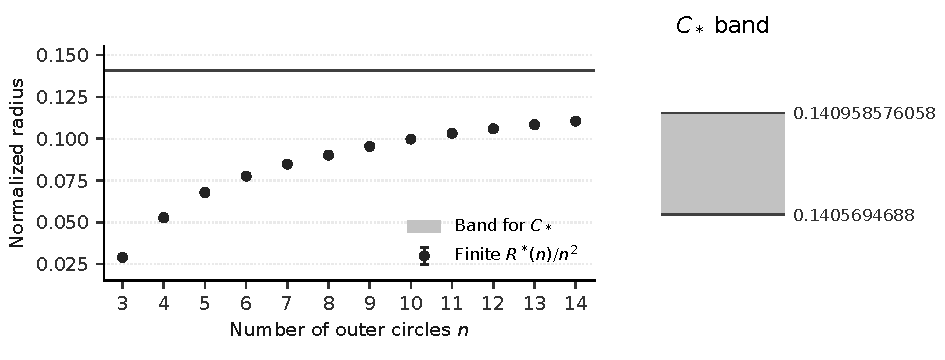
\includegraphics[width=.80\linewidth]{figures/finite_brackets.pdf}
\caption{Certified brackets for $\Rstar(n)/n^2$ from Paper~I
\cite{paperI}. Each interval has width $10^{-11}/n^2$, smaller than
its marker. The dashed line is the rounded lower bound $\CstarLower$
for the limiting coefficient.}
\label{fig:finite}
\end{figure}

Sharper endpoint constructions, tractable evaluation of the finite
linear programs, the structure of optimizing orders and subleading
terms remain open. Bounds on the limiting coefficient alone place
no contact requirements on an individual finite optimizer.

\section*{Data and code availability}

The source deposit for Paper~II contains S1, the standalone proof
and verifier of the terminal-subset lower bound, and S2, the parameter
isolations and all-pairs recovery of the upper construction~\cite{supp}.
The \href{https://github.com/falker47/ringmin/raw/4b3721df8061f1992cfd242df69b1a0643216d8f/paper_assets/paper_ii_journal/source_bundle.zip}{frozen companion ZIP}
includes a claim-to-proof map, a file manifest with source hashes and
build instructions. S1 is preserved from commit
\texttt{75a2f448038d627b2661ea7c9d6fd0fcdb6d33ae}.
Run \texttt{python -I -S verify.py} in \texttt{lower\_supplement/}
or \texttt{python -I -S verify\_math.py} at the archive root for the
aggregate checks. Candidate word-LP solutions are found with SciPy and
checked by exact rational arithmetic. The source of each figure and
its reproduction command are given in the draft package.

\section*{Acknowledgment}
AI assistance was used for proof exploration, software, drafting and
adversarial checks. Responsibility for the mathematical statements and
presentation rests with the author.

\begin{thebibliography}{99}
\small\raggedright
\bibitem{shelf} H. Alt, K. Buchin, S. Chaplick, O. Cheong, P. Kindermann, C. Knauer and F. Stehn, \emph{Placing your Coins on a Shelf}, Journal of Computational Geometry 9 (2018), 312--327.
\href{https://doi.org/10.20382/jocg.v9i1a10}{doi:10.20382/jocg.v9i1a10}.
\bibitem{bhh} J. Beardwood, J. H. Halton and J. M. Hammersley, \emph{The shortest path through many points}, Proceedings of the Cambridge Philosophical Society 55 (1959), 299--327.
\href{https://doi.org/10.1017/s0305004100034095}{doi:10.1017/s0305004100034095}.
\bibitem{burkard} R. E. Burkard, V. G. Deineko, R. van Dal, J. A. A. van der Veen and G. J. Woeginger, \emph{Well-Solvable Special Cases of the Traveling Salesman Problem: A Survey}, SIAM Review 40 (1998), 496--546.
\href{https://doi.org/10.1137/s0036144596297514}{doi:10.1137/s0036144596297514}.
\bibitem{temporal} R. Dechter, I. Meiri and J. Pearl, \emph{Temporal constraint networks}, Artificial Intelligence 49 (1991), 61--95.
\href{https://doi.org/10.1016/0004-3702(91)90006-6}{doi:10.1016/0004-3702(91)90006-6}.
\bibitem{paperI} M. Falconi, \emph{Minimum central circles: chain order, seam obstructions, and exact finite certification}, arXiv:2607.28654v4 (2026).
The \href{https://arxiv.org/abs/2607.28654v1}{original conjecture} is recorded in the first edition.
\href{https://doi.org/10.48550/arXiv.2607.28654}{doi:10.48550/arXiv.2607.28654}.
\bibitem{supp} M. Falconi, \emph{Minimum central circles: an effective characterization of the global asymptotic constant}, arXiv:2609.13630v3 (2026), with supplementary works S1 and S2.
See the \href{https://arxiv.org/src/2609.13630v3}{versioned source deposit} for both supplements.
\href{https://doi.org/10.48550/arXiv.2609.13630}{doi:10.48550/arXiv.2609.13630}.
\bibitem{contact} B. Klemz, M. N\"ollenburg and R. Prutkin, \emph{Recognizing Weighted Disk Contact Graphs}, Lecture Notes in Computer Science 9411 (2015), 433--446.
\href{https://doi.org/10.1007/978-3-319-27261-0_36}{doi:10.1007/978-3-319-27261-0\_36}.
\bibitem{rump} S. M. Rump, \emph{Verification methods: Rigorous results using floating-point arithmetic}, Acta Numerica 19 (2010), 287--449.
\href{https://doi.org/10.1017/s096249291000005x}{doi:10.1017/s096249291000005x}.
\bibitem{steele} J. M. Steele, \emph{Probability Theory and Combinatorial Optimization}, SIAM, 1997.
\href{https://doi.org/10.1137/1.9781611970029}{doi:10.1137/1.9781611970029}.
\bibitem{supnick} F. Supnick, \emph{Extreme Hamiltonian Lines}, Annals of Mathematics 66 (1957).
\href{https://doi.org/10.2307/1970124}{doi:10.2307/1970124}.
\bibitem{tucker} W. Tucker, \emph{Validated Numerics}, Princeton University Press, 2011.
\href{https://doi.org/10.1515/9781400838974}{doi:10.1515/9781400838974}.
\bibitem{walters} P. Walters, \emph{An Introduction to Ergodic Theory}, Springer, 1982.
\href{https://doi.org/10.1007/978-1-4612-5775-2}{doi:10.1007/978-1-4612-5775-2}.
\end{thebibliography}
\end{document}
